Das Selektionsproblem sucht den Median von einem Feld indem es das Feld in Blöcke unterteilt
\begin{figure}[H]\center% Graphic for TeX using PGF
% Title: C:\Users\andregro\Pictures\Diagramm1.dia
% Creator: Dia v0.97.2
% CreationDate: Mon Nov 05 21:46:38 2012
% For: andregro
% \usepackage{tikz}
% The following commands are not supported in PSTricks at present
% We define them conditionally, so when they are implemented,
% this pgf file will use them.
\ifx\du\undefined
  \newlength{\du}
\fi
\setlength{\du}{15\unitlength}
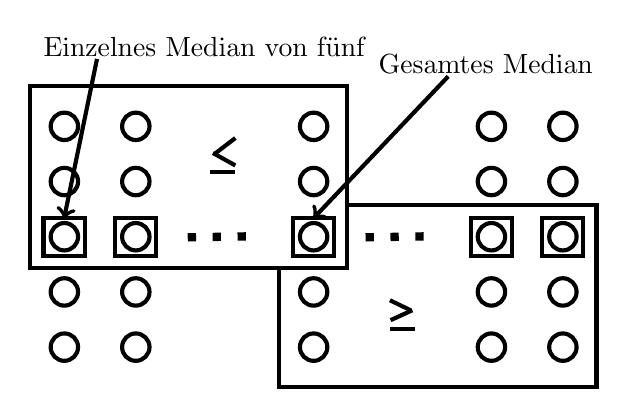
\begin{tikzpicture}[scale=0.6]
\pgftransformxscale{1.000000}
\pgftransformyscale{-1.000000}
\definecolor{dialinecolor}{rgb}{0.000000, 0.000000, 0.000000}
\pgfsetstrokecolor{dialinecolor}
\definecolor{dialinecolor}{rgb}{1.000000, 1.000000, 1.000000}
\pgfsetfillcolor{dialinecolor}
\pgfsetlinewidth{0.100000\du}
\pgfsetdash{}{0pt}
\pgfsetdash{}{0pt}
\pgfsetmiterjoin
\definecolor{dialinecolor}{rgb}{1.000000, 1.000000, 1.000000}
\pgfsetfillcolor{dialinecolor}
\fill (13.105000\du,6.705000\du)--(13.105000\du,14.005000\du)--(25.855000\du,14.005000\du)--(25.855000\du,6.705000\du)--cycle;
\definecolor{dialinecolor}{rgb}{0.000000, 0.000000, 0.000000}
\pgfsetstrokecolor{dialinecolor}
\draw (13.105000\du,6.705000\du)--(13.105000\du,14.005000\du)--(25.855000\du,14.005000\du)--(25.855000\du,6.705000\du)--cycle;
\pgfsetlinewidth{0.100000\du}
\pgfsetdash{}{0pt}
\pgfsetdash{}{0pt}
\pgfsetmiterjoin
\definecolor{dialinecolor}{rgb}{1.000000, 1.000000, 1.000000}
\pgfsetfillcolor{dialinecolor}
\fill (3.100000\du,1.950000\du)--(3.100000\du,9.250000\du)--(15.850000\du,9.250000\du)--(15.850000\du,1.950000\du)--cycle;
\definecolor{dialinecolor}{rgb}{0.000000, 0.000000, 0.000000}
\pgfsetstrokecolor{dialinecolor}
\draw (3.100000\du,1.950000\du)--(3.100000\du,9.250000\du)--(15.850000\du,9.250000\du)--(15.850000\du,1.950000\du)--cycle;
\pgfsetlinewidth{0.100000\du}
\pgfsetdash{}{0pt}
\pgfsetdash{}{0pt}
\pgfsetmiterjoin
\definecolor{dialinecolor}{rgb}{1.000000, 1.000000, 1.000000}
\pgfsetfillcolor{dialinecolor}
\fill (13.662500\du,7.250000\du)--(13.662500\du,8.750000\du)--(15.312500\du,8.750000\du)--(15.312500\du,7.250000\du)--cycle;
\definecolor{dialinecolor}{rgb}{0.000000, 0.000000, 0.000000}
\pgfsetstrokecolor{dialinecolor}
\draw (13.662500\du,7.250000\du)--(13.662500\du,8.750000\du)--(15.312500\du,8.750000\du)--(15.312500\du,7.250000\du)--cycle;
\definecolor{dialinecolor}{rgb}{1.000000, 1.000000, 1.000000}
\pgfsetfillcolor{dialinecolor}
\pgfpathellipse{\pgfpoint{14.497500\du}{7.987500\du}}{\pgfpoint{0.550000\du}{0\du}}{\pgfpoint{0\du}{0.550000\du}}
\pgfusepath{fill}
\pgfsetlinewidth{0.100000\du}
\pgfsetdash{}{0pt}
\pgfsetdash{}{0pt}
\definecolor{dialinecolor}{rgb}{0.000000, 0.000000, 0.000000}
\pgfsetstrokecolor{dialinecolor}
\pgfpathellipse{\pgfpoint{14.497500\du}{7.987500\du}}{\pgfpoint{0.550000\du}{0\du}}{\pgfpoint{0\du}{0.550000\du}}
\pgfusepath{stroke}
\definecolor{dialinecolor}{rgb}{1.000000, 1.000000, 1.000000}
\pgfsetfillcolor{dialinecolor}
\pgfpathellipse{\pgfpoint{14.497500\du}{3.555000\du}}{\pgfpoint{0.550000\du}{0\du}}{\pgfpoint{0\du}{0.550000\du}}
\pgfusepath{fill}
\pgfsetlinewidth{0.100000\du}
\pgfsetdash{}{0pt}
\pgfsetdash{}{0pt}
\definecolor{dialinecolor}{rgb}{0.000000, 0.000000, 0.000000}
\pgfsetstrokecolor{dialinecolor}
\pgfpathellipse{\pgfpoint{14.497500\du}{3.555000\du}}{\pgfpoint{0.550000\du}{0\du}}{\pgfpoint{0\du}{0.550000\du}}
\pgfusepath{stroke}
\definecolor{dialinecolor}{rgb}{1.000000, 1.000000, 1.000000}
\pgfsetfillcolor{dialinecolor}
\pgfpathellipse{\pgfpoint{14.497500\du}{5.771250\du}}{\pgfpoint{0.550000\du}{0\du}}{\pgfpoint{0\du}{0.550000\du}}
\pgfusepath{fill}
\pgfsetlinewidth{0.100000\du}
\pgfsetdash{}{0pt}
\pgfsetdash{}{0pt}
\definecolor{dialinecolor}{rgb}{0.000000, 0.000000, 0.000000}
\pgfsetstrokecolor{dialinecolor}
\pgfpathellipse{\pgfpoint{14.497500\du}{5.771250\du}}{\pgfpoint{0.550000\du}{0\du}}{\pgfpoint{0\du}{0.550000\du}}
\pgfusepath{stroke}
\definecolor{dialinecolor}{rgb}{1.000000, 1.000000, 1.000000}
\pgfsetfillcolor{dialinecolor}
\pgfpathellipse{\pgfpoint{14.497500\du}{10.203750\du}}{\pgfpoint{0.550000\du}{0\du}}{\pgfpoint{0\du}{0.550000\du}}
\pgfusepath{fill}
\pgfsetlinewidth{0.100000\du}
\pgfsetdash{}{0pt}
\pgfsetdash{}{0pt}
\definecolor{dialinecolor}{rgb}{0.000000, 0.000000, 0.000000}
\pgfsetstrokecolor{dialinecolor}
\pgfpathellipse{\pgfpoint{14.497500\du}{10.203750\du}}{\pgfpoint{0.550000\du}{0\du}}{\pgfpoint{0\du}{0.550000\du}}
\pgfusepath{stroke}
\definecolor{dialinecolor}{rgb}{1.000000, 1.000000, 1.000000}
\pgfsetfillcolor{dialinecolor}
\pgfpathellipse{\pgfpoint{14.497500\du}{12.420000\du}}{\pgfpoint{0.550000\du}{0\du}}{\pgfpoint{0\du}{0.550000\du}}
\pgfusepath{fill}
\pgfsetlinewidth{0.100000\du}
\pgfsetdash{}{0pt}
\pgfsetdash{}{0pt}
\definecolor{dialinecolor}{rgb}{0.000000, 0.000000, 0.000000}
\pgfsetstrokecolor{dialinecolor}
\pgfpathellipse{\pgfpoint{14.497500\du}{12.420000\du}}{\pgfpoint{0.550000\du}{0\du}}{\pgfpoint{0\du}{0.550000\du}}
\pgfusepath{stroke}
\pgfsetlinewidth{0.100000\du}
\pgfsetdash{}{0pt}
\pgfsetdash{}{0pt}
\pgfsetmiterjoin
\definecolor{dialinecolor}{rgb}{1.000000, 1.000000, 1.000000}
\pgfsetfillcolor{dialinecolor}
\fill (3.655000\du,7.250000\du)--(3.655000\du,8.750000\du)--(5.305000\du,8.750000\du)--(5.305000\du,7.250000\du)--cycle;
\definecolor{dialinecolor}{rgb}{0.000000, 0.000000, 0.000000}
\pgfsetstrokecolor{dialinecolor}
\draw (3.655000\du,7.250000\du)--(3.655000\du,8.750000\du)--(5.305000\du,8.750000\du)--(5.305000\du,7.250000\du)--cycle;
\definecolor{dialinecolor}{rgb}{1.000000, 1.000000, 1.000000}
\pgfsetfillcolor{dialinecolor}
\pgfpathellipse{\pgfpoint{4.490000\du}{7.987500\du}}{\pgfpoint{0.550000\du}{0\du}}{\pgfpoint{0\du}{0.550000\du}}
\pgfusepath{fill}
\pgfsetlinewidth{0.100000\du}
\pgfsetdash{}{0pt}
\pgfsetdash{}{0pt}
\definecolor{dialinecolor}{rgb}{0.000000, 0.000000, 0.000000}
\pgfsetstrokecolor{dialinecolor}
\pgfpathellipse{\pgfpoint{4.490000\du}{7.987500\du}}{\pgfpoint{0.550000\du}{0\du}}{\pgfpoint{0\du}{0.550000\du}}
\pgfusepath{stroke}
\definecolor{dialinecolor}{rgb}{1.000000, 1.000000, 1.000000}
\pgfsetfillcolor{dialinecolor}
\pgfpathellipse{\pgfpoint{4.490000\du}{3.555000\du}}{\pgfpoint{0.550000\du}{0\du}}{\pgfpoint{0\du}{0.550000\du}}
\pgfusepath{fill}
\pgfsetlinewidth{0.100000\du}
\pgfsetdash{}{0pt}
\pgfsetdash{}{0pt}
\definecolor{dialinecolor}{rgb}{0.000000, 0.000000, 0.000000}
\pgfsetstrokecolor{dialinecolor}
\pgfpathellipse{\pgfpoint{4.490000\du}{3.555000\du}}{\pgfpoint{0.550000\du}{0\du}}{\pgfpoint{0\du}{0.550000\du}}
\pgfusepath{stroke}
\definecolor{dialinecolor}{rgb}{1.000000, 1.000000, 1.000000}
\pgfsetfillcolor{dialinecolor}
\pgfpathellipse{\pgfpoint{4.490000\du}{5.771250\du}}{\pgfpoint{0.550000\du}{0\du}}{\pgfpoint{0\du}{0.550000\du}}
\pgfusepath{fill}
\pgfsetlinewidth{0.100000\du}
\pgfsetdash{}{0pt}
\pgfsetdash{}{0pt}
\definecolor{dialinecolor}{rgb}{0.000000, 0.000000, 0.000000}
\pgfsetstrokecolor{dialinecolor}
\pgfpathellipse{\pgfpoint{4.490000\du}{5.771250\du}}{\pgfpoint{0.550000\du}{0\du}}{\pgfpoint{0\du}{0.550000\du}}
\pgfusepath{stroke}
\definecolor{dialinecolor}{rgb}{1.000000, 1.000000, 1.000000}
\pgfsetfillcolor{dialinecolor}
\pgfpathellipse{\pgfpoint{4.490000\du}{10.203750\du}}{\pgfpoint{0.550000\du}{0\du}}{\pgfpoint{0\du}{0.550000\du}}
\pgfusepath{fill}
\pgfsetlinewidth{0.100000\du}
\pgfsetdash{}{0pt}
\pgfsetdash{}{0pt}
\definecolor{dialinecolor}{rgb}{0.000000, 0.000000, 0.000000}
\pgfsetstrokecolor{dialinecolor}
\pgfpathellipse{\pgfpoint{4.490000\du}{10.203750\du}}{\pgfpoint{0.550000\du}{0\du}}{\pgfpoint{0\du}{0.550000\du}}
\pgfusepath{stroke}
\definecolor{dialinecolor}{rgb}{1.000000, 1.000000, 1.000000}
\pgfsetfillcolor{dialinecolor}
\pgfpathellipse{\pgfpoint{4.490000\du}{12.420000\du}}{\pgfpoint{0.550000\du}{0\du}}{\pgfpoint{0\du}{0.550000\du}}
\pgfusepath{fill}
\pgfsetlinewidth{0.100000\du}
\pgfsetdash{}{0pt}
\pgfsetdash{}{0pt}
\definecolor{dialinecolor}{rgb}{0.000000, 0.000000, 0.000000}
\pgfsetstrokecolor{dialinecolor}
\pgfpathellipse{\pgfpoint{4.490000\du}{12.420000\du}}{\pgfpoint{0.550000\du}{0\du}}{\pgfpoint{0\du}{0.550000\du}}
\pgfusepath{stroke}
\pgfsetlinewidth{0.100000\du}
\pgfsetdash{}{0pt}
\pgfsetdash{}{0pt}
\pgfsetmiterjoin
\definecolor{dialinecolor}{rgb}{1.000000, 1.000000, 1.000000}
\pgfsetfillcolor{dialinecolor}
\fill (6.523050\du,7.250000\du)--(6.523050\du,8.750000\du)--(8.173050\du,8.750000\du)--(8.173050\du,7.250000\du)--cycle;
\definecolor{dialinecolor}{rgb}{0.000000, 0.000000, 0.000000}
\pgfsetstrokecolor{dialinecolor}
\draw (6.523050\du,7.250000\du)--(6.523050\du,8.750000\du)--(8.173050\du,8.750000\du)--(8.173050\du,7.250000\du)--cycle;
\definecolor{dialinecolor}{rgb}{1.000000, 1.000000, 1.000000}
\pgfsetfillcolor{dialinecolor}
\pgfpathellipse{\pgfpoint{7.358050\du}{7.987500\du}}{\pgfpoint{0.550000\du}{0\du}}{\pgfpoint{0\du}{0.550000\du}}
\pgfusepath{fill}
\pgfsetlinewidth{0.100000\du}
\pgfsetdash{}{0pt}
\pgfsetdash{}{0pt}
\definecolor{dialinecolor}{rgb}{0.000000, 0.000000, 0.000000}
\pgfsetstrokecolor{dialinecolor}
\pgfpathellipse{\pgfpoint{7.358050\du}{7.987500\du}}{\pgfpoint{0.550000\du}{0\du}}{\pgfpoint{0\du}{0.550000\du}}
\pgfusepath{stroke}
\definecolor{dialinecolor}{rgb}{1.000000, 1.000000, 1.000000}
\pgfsetfillcolor{dialinecolor}
\pgfpathellipse{\pgfpoint{7.358050\du}{3.555000\du}}{\pgfpoint{0.550000\du}{0\du}}{\pgfpoint{0\du}{0.550000\du}}
\pgfusepath{fill}
\pgfsetlinewidth{0.100000\du}
\pgfsetdash{}{0pt}
\pgfsetdash{}{0pt}
\definecolor{dialinecolor}{rgb}{0.000000, 0.000000, 0.000000}
\pgfsetstrokecolor{dialinecolor}
\pgfpathellipse{\pgfpoint{7.358050\du}{3.555000\du}}{\pgfpoint{0.550000\du}{0\du}}{\pgfpoint{0\du}{0.550000\du}}
\pgfusepath{stroke}
\definecolor{dialinecolor}{rgb}{1.000000, 1.000000, 1.000000}
\pgfsetfillcolor{dialinecolor}
\pgfpathellipse{\pgfpoint{7.358050\du}{5.771250\du}}{\pgfpoint{0.550000\du}{0\du}}{\pgfpoint{0\du}{0.550000\du}}
\pgfusepath{fill}
\pgfsetlinewidth{0.100000\du}
\pgfsetdash{}{0pt}
\pgfsetdash{}{0pt}
\definecolor{dialinecolor}{rgb}{0.000000, 0.000000, 0.000000}
\pgfsetstrokecolor{dialinecolor}
\pgfpathellipse{\pgfpoint{7.358050\du}{5.771250\du}}{\pgfpoint{0.550000\du}{0\du}}{\pgfpoint{0\du}{0.550000\du}}
\pgfusepath{stroke}
\definecolor{dialinecolor}{rgb}{1.000000, 1.000000, 1.000000}
\pgfsetfillcolor{dialinecolor}
\pgfpathellipse{\pgfpoint{7.358050\du}{10.203750\du}}{\pgfpoint{0.550000\du}{0\du}}{\pgfpoint{0\du}{0.550000\du}}
\pgfusepath{fill}
\pgfsetlinewidth{0.100000\du}
\pgfsetdash{}{0pt}
\pgfsetdash{}{0pt}
\definecolor{dialinecolor}{rgb}{0.000000, 0.000000, 0.000000}
\pgfsetstrokecolor{dialinecolor}
\pgfpathellipse{\pgfpoint{7.358050\du}{10.203750\du}}{\pgfpoint{0.550000\du}{0\du}}{\pgfpoint{0\du}{0.550000\du}}
\pgfusepath{stroke}
\definecolor{dialinecolor}{rgb}{1.000000, 1.000000, 1.000000}
\pgfsetfillcolor{dialinecolor}
\pgfpathellipse{\pgfpoint{7.358050\du}{12.420000\du}}{\pgfpoint{0.550000\du}{0\du}}{\pgfpoint{0\du}{0.550000\du}}
\pgfusepath{fill}
\pgfsetlinewidth{0.100000\du}
\pgfsetdash{}{0pt}
\pgfsetdash{}{0pt}
\definecolor{dialinecolor}{rgb}{0.000000, 0.000000, 0.000000}
\pgfsetstrokecolor{dialinecolor}
\pgfpathellipse{\pgfpoint{7.358050\du}{12.420000\du}}{\pgfpoint{0.550000\du}{0\du}}{\pgfpoint{0\du}{0.550000\du}}
\pgfusepath{stroke}
\pgfsetlinewidth{0.100000\du}
\pgfsetdash{}{0pt}
\pgfsetdash{}{0pt}
\pgfsetmiterjoin
\definecolor{dialinecolor}{rgb}{1.000000, 1.000000, 1.000000}
\pgfsetfillcolor{dialinecolor}
\fill (20.802000\du,7.250000\du)--(20.802000\du,8.750000\du)--(22.452000\du,8.750000\du)--(22.452000\du,7.250000\du)--cycle;
\definecolor{dialinecolor}{rgb}{0.000000, 0.000000, 0.000000}
\pgfsetstrokecolor{dialinecolor}
\draw (20.802000\du,7.250000\du)--(20.802000\du,8.750000\du)--(22.452000\du,8.750000\du)--(22.452000\du,7.250000\du)--cycle;
\definecolor{dialinecolor}{rgb}{1.000000, 1.000000, 1.000000}
\pgfsetfillcolor{dialinecolor}
\pgfpathellipse{\pgfpoint{21.637000\du}{7.987500\du}}{\pgfpoint{0.550000\du}{0\du}}{\pgfpoint{0\du}{0.550000\du}}
\pgfusepath{fill}
\pgfsetlinewidth{0.100000\du}
\pgfsetdash{}{0pt}
\pgfsetdash{}{0pt}
\definecolor{dialinecolor}{rgb}{0.000000, 0.000000, 0.000000}
\pgfsetstrokecolor{dialinecolor}
\pgfpathellipse{\pgfpoint{21.637000\du}{7.987500\du}}{\pgfpoint{0.550000\du}{0\du}}{\pgfpoint{0\du}{0.550000\du}}
\pgfusepath{stroke}
\definecolor{dialinecolor}{rgb}{1.000000, 1.000000, 1.000000}
\pgfsetfillcolor{dialinecolor}
\pgfpathellipse{\pgfpoint{21.637000\du}{3.555000\du}}{\pgfpoint{0.550000\du}{0\du}}{\pgfpoint{0\du}{0.550000\du}}
\pgfusepath{fill}
\pgfsetlinewidth{0.100000\du}
\pgfsetdash{}{0pt}
\pgfsetdash{}{0pt}
\definecolor{dialinecolor}{rgb}{0.000000, 0.000000, 0.000000}
\pgfsetstrokecolor{dialinecolor}
\pgfpathellipse{\pgfpoint{21.637000\du}{3.555000\du}}{\pgfpoint{0.550000\du}{0\du}}{\pgfpoint{0\du}{0.550000\du}}
\pgfusepath{stroke}
\definecolor{dialinecolor}{rgb}{1.000000, 1.000000, 1.000000}
\pgfsetfillcolor{dialinecolor}
\pgfpathellipse{\pgfpoint{21.637000\du}{5.771250\du}}{\pgfpoint{0.550000\du}{0\du}}{\pgfpoint{0\du}{0.550000\du}}
\pgfusepath{fill}
\pgfsetlinewidth{0.100000\du}
\pgfsetdash{}{0pt}
\pgfsetdash{}{0pt}
\definecolor{dialinecolor}{rgb}{0.000000, 0.000000, 0.000000}
\pgfsetstrokecolor{dialinecolor}
\pgfpathellipse{\pgfpoint{21.637000\du}{5.771250\du}}{\pgfpoint{0.550000\du}{0\du}}{\pgfpoint{0\du}{0.550000\du}}
\pgfusepath{stroke}
\definecolor{dialinecolor}{rgb}{1.000000, 1.000000, 1.000000}
\pgfsetfillcolor{dialinecolor}
\pgfpathellipse{\pgfpoint{21.637000\du}{10.203750\du}}{\pgfpoint{0.550000\du}{0\du}}{\pgfpoint{0\du}{0.550000\du}}
\pgfusepath{fill}
\pgfsetlinewidth{0.100000\du}
\pgfsetdash{}{0pt}
\pgfsetdash{}{0pt}
\definecolor{dialinecolor}{rgb}{0.000000, 0.000000, 0.000000}
\pgfsetstrokecolor{dialinecolor}
\pgfpathellipse{\pgfpoint{21.637000\du}{10.203750\du}}{\pgfpoint{0.550000\du}{0\du}}{\pgfpoint{0\du}{0.550000\du}}
\pgfusepath{stroke}
\definecolor{dialinecolor}{rgb}{1.000000, 1.000000, 1.000000}
\pgfsetfillcolor{dialinecolor}
\pgfpathellipse{\pgfpoint{21.637000\du}{12.420000\du}}{\pgfpoint{0.550000\du}{0\du}}{\pgfpoint{0\du}{0.550000\du}}
\pgfusepath{fill}
\pgfsetlinewidth{0.100000\du}
\pgfsetdash{}{0pt}
\pgfsetdash{}{0pt}
\definecolor{dialinecolor}{rgb}{0.000000, 0.000000, 0.000000}
\pgfsetstrokecolor{dialinecolor}
\pgfpathellipse{\pgfpoint{21.637000\du}{12.420000\du}}{\pgfpoint{0.550000\du}{0\du}}{\pgfpoint{0\du}{0.550000\du}}
\pgfusepath{stroke}
\pgfsetlinewidth{0.100000\du}
\pgfsetdash{}{0pt}
\pgfsetdash{}{0pt}
\pgfsetmiterjoin
\definecolor{dialinecolor}{rgb}{1.000000, 1.000000, 1.000000}
\pgfsetfillcolor{dialinecolor}
\fill (23.670000\du,7.250000\du)--(23.670000\du,8.750000\du)--(25.320000\du,8.750000\du)--(25.320000\du,7.250000\du)--cycle;
\definecolor{dialinecolor}{rgb}{0.000000, 0.000000, 0.000000}
\pgfsetstrokecolor{dialinecolor}
\draw (23.670000\du,7.250000\du)--(23.670000\du,8.750000\du)--(25.320000\du,8.750000\du)--(25.320000\du,7.250000\du)--cycle;
\definecolor{dialinecolor}{rgb}{1.000000, 1.000000, 1.000000}
\pgfsetfillcolor{dialinecolor}
\pgfpathellipse{\pgfpoint{24.505000\du}{7.987500\du}}{\pgfpoint{0.550000\du}{0\du}}{\pgfpoint{0\du}{0.550000\du}}
\pgfusepath{fill}
\pgfsetlinewidth{0.100000\du}
\pgfsetdash{}{0pt}
\pgfsetdash{}{0pt}
\definecolor{dialinecolor}{rgb}{0.000000, 0.000000, 0.000000}
\pgfsetstrokecolor{dialinecolor}
\pgfpathellipse{\pgfpoint{24.505000\du}{7.987500\du}}{\pgfpoint{0.550000\du}{0\du}}{\pgfpoint{0\du}{0.550000\du}}
\pgfusepath{stroke}
\definecolor{dialinecolor}{rgb}{1.000000, 1.000000, 1.000000}
\pgfsetfillcolor{dialinecolor}
\pgfpathellipse{\pgfpoint{24.505000\du}{3.555000\du}}{\pgfpoint{0.550000\du}{0\du}}{\pgfpoint{0\du}{0.550000\du}}
\pgfusepath{fill}
\pgfsetlinewidth{0.100000\du}
\pgfsetdash{}{0pt}
\pgfsetdash{}{0pt}
\definecolor{dialinecolor}{rgb}{0.000000, 0.000000, 0.000000}
\pgfsetstrokecolor{dialinecolor}
\pgfpathellipse{\pgfpoint{24.505000\du}{3.555000\du}}{\pgfpoint{0.550000\du}{0\du}}{\pgfpoint{0\du}{0.550000\du}}
\pgfusepath{stroke}
\definecolor{dialinecolor}{rgb}{1.000000, 1.000000, 1.000000}
\pgfsetfillcolor{dialinecolor}
\pgfpathellipse{\pgfpoint{24.505000\du}{5.771250\du}}{\pgfpoint{0.550000\du}{0\du}}{\pgfpoint{0\du}{0.550000\du}}
\pgfusepath{fill}
\pgfsetlinewidth{0.100000\du}
\pgfsetdash{}{0pt}
\pgfsetdash{}{0pt}
\definecolor{dialinecolor}{rgb}{0.000000, 0.000000, 0.000000}
\pgfsetstrokecolor{dialinecolor}
\pgfpathellipse{\pgfpoint{24.505000\du}{5.771250\du}}{\pgfpoint{0.550000\du}{0\du}}{\pgfpoint{0\du}{0.550000\du}}
\pgfusepath{stroke}
\definecolor{dialinecolor}{rgb}{1.000000, 1.000000, 1.000000}
\pgfsetfillcolor{dialinecolor}
\pgfpathellipse{\pgfpoint{24.505000\du}{10.203750\du}}{\pgfpoint{0.550000\du}{0\du}}{\pgfpoint{0\du}{0.550000\du}}
\pgfusepath{fill}
\pgfsetlinewidth{0.100000\du}
\pgfsetdash{}{0pt}
\pgfsetdash{}{0pt}
\definecolor{dialinecolor}{rgb}{0.000000, 0.000000, 0.000000}
\pgfsetstrokecolor{dialinecolor}
\pgfpathellipse{\pgfpoint{24.505000\du}{10.203750\du}}{\pgfpoint{0.550000\du}{0\du}}{\pgfpoint{0\du}{0.550000\du}}
\pgfusepath{stroke}
\definecolor{dialinecolor}{rgb}{1.000000, 1.000000, 1.000000}
\pgfsetfillcolor{dialinecolor}
\pgfpathellipse{\pgfpoint{24.505000\du}{12.420000\du}}{\pgfpoint{0.550000\du}{0\du}}{\pgfpoint{0\du}{0.550000\du}}
\pgfusepath{fill}
\pgfsetlinewidth{0.100000\du}
\pgfsetdash{}{0pt}
\pgfsetdash{}{0pt}
\definecolor{dialinecolor}{rgb}{0.000000, 0.000000, 0.000000}
\pgfsetstrokecolor{dialinecolor}
\pgfpathellipse{\pgfpoint{24.505000\du}{12.420000\du}}{\pgfpoint{0.550000\du}{0\du}}{\pgfpoint{0\du}{0.550000\du}}
\pgfusepath{stroke}
\pgfsetlinewidth{0.200000\du}
\pgfsetdash{{\pgflinewidth}{0.200000\du}}{0cm}
\pgfsetdash{{\pgflinewidth}{0.400000\du}}{0cm}
\pgfsetbuttcap
{
\definecolor{dialinecolor}{rgb}{0.000000, 0.000000, 0.000000}
\pgfsetfillcolor{dialinecolor}
% was here!!!
\definecolor{dialinecolor}{rgb}{0.000000, 0.000000, 0.000000}
\pgfsetstrokecolor{dialinecolor}
\draw (16.582200\du,8.012500\du)--(19.532200\du,7.962500\du);
}
\pgfsetlinewidth{0.200000\du}
\pgfsetdash{{\pgflinewidth}{0.400000\du}}{0cm}
\pgfsetdash{{\pgflinewidth}{0.400000\du}}{0cm}
\pgfsetbuttcap
{
\definecolor{dialinecolor}{rgb}{0.000000, 0.000000, 0.000000}
\pgfsetfillcolor{dialinecolor}
% was here!!!
\definecolor{dialinecolor}{rgb}{0.000000, 0.000000, 0.000000}
\pgfsetstrokecolor{dialinecolor}
\draw (9.442770\du,8.012500\du)--(12.392800\du,7.962500\du);
}
\pgfsetlinewidth{0.100000\du}
\pgfsetdash{}{0pt}
\pgfsetdash{}{0pt}
\pgfsetbuttcap
{
\definecolor{dialinecolor}{rgb}{0.000000, 0.000000, 0.000000}
\pgfsetfillcolor{dialinecolor}
% was here!!!
\pgfsetarrowsstart{to}
\definecolor{dialinecolor}{rgb}{0.000000, 0.000000, 0.000000}
\pgfsetstrokecolor{dialinecolor}
\draw (14.487500\du,7.250000\du)--(19.900000\du,1.550000\du);
}
\pgfsetlinewidth{0.100000\du}
\pgfsetdash{}{0pt}
\pgfsetdash{}{0pt}
\pgfsetbuttcap
{
\definecolor{dialinecolor}{rgb}{0.000000, 0.000000, 0.000000}
\pgfsetfillcolor{dialinecolor}
% was here!!!
\pgfsetarrowsstart{to}
\definecolor{dialinecolor}{rgb}{0.000000, 0.000000, 0.000000}
\pgfsetstrokecolor{dialinecolor}
\draw (4.480000\du,7.250000\du)--(5.800000\du,0.850000\du);
}
% setfont left to latex
\definecolor{dialinecolor}{rgb}{0.000000, 0.000000, 0.000000}
\pgfsetstrokecolor{dialinecolor}
\node[anchor=west] at (3.200000\du,0.350000\du){Einzelnes Median von fünf};
% setfont left to latex
\definecolor{dialinecolor}{rgb}{0.000000, 0.000000, 0.000000}
\pgfsetstrokecolor{dialinecolor}
\node[anchor=west] at (16.655000\du,1.067500\du){Gesamtes Median};
\pgfsetlinewidth{0.100000\du}
\pgfsetdash{}{0pt}
\pgfsetdash{}{0pt}
\pgfsetbuttcap
{
\definecolor{dialinecolor}{rgb}{0.000000, 0.000000, 0.000000}
\pgfsetfillcolor{dialinecolor}
% was here!!!
\definecolor{dialinecolor}{rgb}{0.000000, 0.000000, 0.000000}
\pgfsetstrokecolor{dialinecolor}
\draw (11.355000\du,4.025090\du)--(10.505000\du,4.675090\du);
}
\pgfsetlinewidth{0.100000\du}
\pgfsetdash{}{0pt}
\pgfsetdash{}{0pt}
\pgfsetbuttcap
{
\definecolor{dialinecolor}{rgb}{0.000000, 0.000000, 0.000000}
\pgfsetfillcolor{dialinecolor}
% was here!!!
\definecolor{dialinecolor}{rgb}{0.000000, 0.000000, 0.000000}
\pgfsetstrokecolor{dialinecolor}
\draw (10.455000\du,4.625090\du)--(11.355000\du,5.125090\du);
}
\pgfsetlinewidth{0.100000\du}
\pgfsetdash{}{0pt}
\pgfsetdash{}{0pt}
\pgfsetbuttcap
{
\definecolor{dialinecolor}{rgb}{0.000000, 0.000000, 0.000000}
\pgfsetfillcolor{dialinecolor}
% was here!!!
\definecolor{dialinecolor}{rgb}{0.000000, 0.000000, 0.000000}
\pgfsetstrokecolor{dialinecolor}
\draw (10.355000\du,5.375090\du)--(11.355000\du,5.375090\du);
}
\pgfsetlinewidth{0.100000\du}
\pgfsetdash{}{0pt}
\pgfsetdash{}{0pt}
\pgfsetbuttcap
{
\definecolor{dialinecolor}{rgb}{0.000000, 0.000000, 0.000000}
\pgfsetfillcolor{dialinecolor}
% was here!!!
\definecolor{dialinecolor}{rgb}{0.000000, 0.000000, 0.000000}
\pgfsetstrokecolor{dialinecolor}
\draw (17.562500\du,10.537500\du)--(18.387500\du,10.937500\du);
}
\pgfsetlinewidth{0.100000\du}
\pgfsetdash{}{0pt}
\pgfsetdash{}{0pt}
\pgfsetbuttcap
{
\definecolor{dialinecolor}{rgb}{0.000000, 0.000000, 0.000000}
\pgfsetfillcolor{dialinecolor}
% was here!!!
\definecolor{dialinecolor}{rgb}{0.000000, 0.000000, 0.000000}
\pgfsetstrokecolor{dialinecolor}
\draw (18.462500\du,10.937500\du)--(17.587500\du,11.337500\du);
}
\pgfsetlinewidth{0.100000\du}
\pgfsetdash{}{0pt}
\pgfsetdash{}{0pt}
\pgfsetbuttcap
{
\definecolor{dialinecolor}{rgb}{0.000000, 0.000000, 0.000000}
\pgfsetfillcolor{dialinecolor}
% was here!!!
\definecolor{dialinecolor}{rgb}{0.000000, 0.000000, 0.000000}
\pgfsetstrokecolor{dialinecolor}
\draw (17.550000\du,11.700000\du)--(18.550000\du,11.700000\du);
}
\end{tikzpicture}
\caption{Selektionsproblem}\end{figure}
$\frac{3n}{10}$ der Elemente sind$\le M$\\
$$T(n)=cn+T\left(\frac{n}{5}\right)+T\left(\frac{7n}{10}\right)$$
Akra Bazzi Theorem:
\begin{align*}
T(n)&=\sum_{i=1}^ka_iT\left(\frac{n}{b_i}+g(n)\right)\\
\Rightarrow T(n)&= \mathcal O\left( n^p\left(1+\int_1^n\frac{g(u)}{u^{p+1}}du\right)\right)\\
T(n)&=\mathcal O\left(n^p\left(1+\int_1^n\frac{cu}{u^{p+1}}du\right)\right)\\
&=\mathcal O\left(n^p\left(1+\frac{c}{1-p}n^{-p+1}\right)\right)\\
&=\mathcal O(n^p+n^1)=\mathcal O(n)
\end{align*}
\fbox{\parbox{\columnwidth}{Nebenrechnung:\small\begin{align*}&\sum_{i=1}^k\frac{a_i}{b_i^p}=1\\
&g(n)=cn\\
&a_1=a_2=1;\,b_1=5;\, b_2=\frac{10}{7}\\
&\left( \frac{1}{5} \right)^p+ \left( \frac{7}{10} \right)^p=1\\
&p\approx 0,84 \le 1\end{align*}}}\\[.5em]